\section{Domain Background}
A central goal in evolutionary research is to understand the trajectory evolution took in the past and predict the trajectories it is likely to take in the future. 
Both the reconstruction of the past and prediction of the future require a strong working model of the evolutionary search space; that is, what combinations of traits might an organism have, and how do those combinations lead to reproductive success or failure? 
Consider as a simplifeid example the fitness of a tree; two traits of interest might be the depth and breadth of its root system.
One might be able to quantify the fitness impacts of these two traits and write an optimization function to find the maximum. 
Finding the maximum fitness, however, is of limited use when you don't know if evolution can actually find the necessary combination of traits; an extremely deep and extremely wide root system might be helpful, but also energetically infeasible.
Thus, it is frequently much more important to understand the trajectory that evolution will take through the problem space.
Such knowledge is particularly critical for efforts to prevent the evolution of dangerous traits (\textit{e.g.} antibiotic resistant bacteria) by precisely controlling the trajectory of evolution \citep{iram_controlling_2021}.
It is therefore useful to have some way to visualize the entire domain of the traits of interest as they relate to fitness.

\begin{figure}
    \centering
    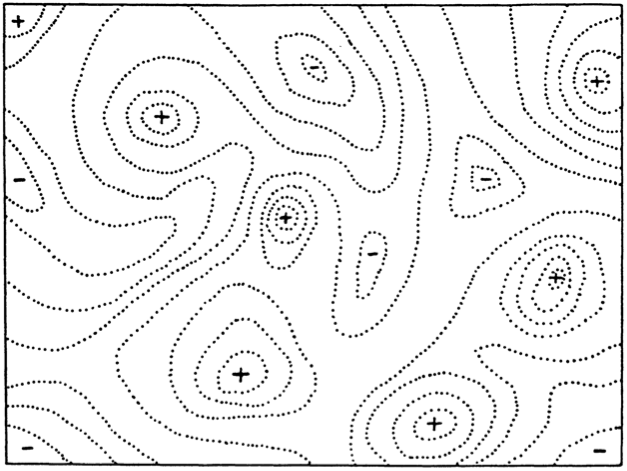
\includegraphics[width=0.5\textwidth]{chapters/3-vr-viz/figs/wright.png}
    \caption{Original fitness landscape schematic from Wright (1932). Plus signs represent peaks while minus signs represent valleys. Dotted lines indicate changes in altitude (that is, changes in fitness).}
    \label{fig:bkg:wright}
\end{figure}

\subsection{Evolutionary Fitness Landscapes}
The current predominant method of visualizing the evolutionary search space is the \textit{evolutionary fitness landscape}. 
This visual metaphor, created by Sewall Wright \citep{wright_roles_1932}, depicts two traits as $x$ and $y$ coordinates with fitness as a third $z$ coordinate, often represented as height (\autoref{fig:bkg:wright}). 
The result is indeed a landscape-like appearance, which brings a sense of intuitive familiarity to the reader; higher fitness areas are easy to spot, and movement around the space is easy to imagine. 

Such a familiar depiction has made fitness landscapes a nearly ubiquitous visual metaphor. 
Evolution research across fields frequently uses the terms ``peaks" and ``valleys" to describe areas of high and low fitness respectively. 
Furthermore, populations moving from low-fitness regions to high-fitness regions are said to be ``hill-climbing", while populations moving through low-fitness regions are ``valley-crossing". 
These terms and the image of the underlying landscape are descriptive and easily understandable; unfortunately, they can also be severely misleading as to the true nature of evolutionary space.

\subsection{Loss of Information \& Intuition}

One obvious shortcoming of the topographical fitness landscape is that it depicts only two traits and therefore encourages imagination of the evolutionary space in only three dimensions. 
However, most real-world evolutionary spaces are extremely high-dimensional; any trait an organism possesses might be considered a dimension of the evolutionary landscape. 
Some conceptualizations go even farther, treating the identity of the nucleotide at each position in an organism's DNA sequence as a separate dimension. 
Intuition about movement across low-dimensional spaces does not always translate well to intuition about similar movement across high-dimensional spaces \citep{agarwala_adaptive_2019}; therefore, relying on 2D visual landscape metaphors can mislead us about certain evolutionary dynamics.

One such evolutionary dynamic of particular interest is the aforementioned \textit{valley-crossing} problem. In the fitness landscape metaphor, both local and global maxima are represented as peaks. At one of these peaks, any small mutation of a trait will necessarily shift the population to an area of lower fitness, and evolutionary pressure will then return the population to the peak. How then are populations able to move from local maxima to global maxima when they are effectively buffeted away from moving through the intervening areas of low fitness?

Research inspired by intuitions from low-dimensional landscapes tends to approach this problem with the implicit assumption that valley crossing requires 1) multiple mutations to occur at once, or 2) a sequence of individuals with deleterious (\textit{i.e.} fitness-reducing) mutations to survive long enough to have an offspring that lands on the opposite side of the valley. Much effort has been devoted to understanding what conditions allow these scenarios. However, researchers skilled in understanding the mathematical properties of high-dimensional landscapes have suggested that this is the wrong question \citep{kaplan_end_2008, gavrilets_2010}. In high dimensional spaces, they argue, the probability of a valley existing in all dimensions simultaneously is very low. In this view, populations do not need to cross valleys and instead likely drift across neutral ``ridges'' between the peaks. This phenomenon is sometimes referred to as an ``extradimensional bypass'' -- a path along one dimension that connects two peaks \citep{cariani_extradimensional_2002}. %Another approach 

%There are multiple good explanations of how populations undergo or avoid valley-crossing, such as imagining landscapes as ``holey" binary surfaces rather than topographies, or identifying multiple mutations which could ``launch" organisms from peak to peak across valleys. However, one simple explanation is that our intuitive, fitness landscape based idea of ``fitness valleys" is itself problematic; in high-dimensional spaces, ``peaks" may be so frequent and so close together in evolutionary space that valley crossing presents no problem if mutations are of any appreciable size (CITE). 

In this case, it would seem that attempts to visualize fitness landscapes as three-dimensional surfaces are not aiding scientific discovery and are in fact hindering our understanding. This issue has been well-known for over a decade and is severe enough that some domain experts have called for an end to the fitness landscape metaphor altogether \citep{kaplan_end_2008}, but the metaphor remains popular. Many people think most clearly about problems when they have a thorough mental image of them. Asking them to abandon that mental image without providing a better replacement is not an ideal solution. Thus, we suggest that the most beneficial next step for the community is to build an improved intuition for the ways in which low-dimensional fitness landscape visualizations may mislead us. If the fitness landscape metaphor is to continue being used, evolutionary scientists need a visceral understanding of where it is useful and where it falls short. Here, we seek to do exactly that. 

\subsection{Holey fitness landscapes}

Another influential way of thinking about high-dimensional fitness landscapes, is the idea of holey fitness landscapes \citep{gavrilets_evolution_1997}. This concept is inspired by the idea that, in realistic fitness landscapes, nearly all high-fitness genotypes are mutationally adjacent to other genotypes of comparable fitness. Thus, it may be useful to abstract a high dimensional landscape by compressing the space of possible fitnesses to two: viable and not viable. The resulting search space can be visualized as a plateau (the viable genotypes) with holes cut out of it (the not viable genotypes). Evolution in such a space is a matter of neutral diffusion along the plateau, and can be modeled as a percolation process \citep{gavrilets_high-dimensional_2010}.

While this model has been criticized both for abstracting away important dynamics and for being misleading in its own way \citep{kaplan_end_2008}, it has so strongly influenced thinking on how best to conceptualize high-dimensional fitness landscapes that we would feel remiss in not mentioning it here. Although we have yet to explicitly incorporate this thinking into Tessevolve, it suggests a variety of valuable future directions.